% \documentclass[handout]{beamer}
\documentclass{beamer}

\mode<presentation>
{
  \usetheme{default}
  \usefonttheme[onlymath]{serif}
  % \usetheme{Singapore}
  % \usetheme{Warsaw}
  % \usetheme{Malmoe}
  % \useinnertheme{circles}
  % \useoutertheme{infolines}
  % \useinnertheme{rounded}

  \setbeamercovered{transparent=100}
}

\usepackage[english]{babel}
\usepackage[latin1]{inputenc}
\usepackage{alltt,listings,multirow,ulem,siunitx}
\usepackage[absolute,overlay]{textpos}
\TPGrid{1}{1}
\usepackage{pdfpages}
\usepackage{multimedia}
\usepackage{multicol}
\newcommand\hmmax{0}
\newcommand\bmmax{0}
\usepackage{bm}
\usepackage{comment}

% font definitions, try \usepackage{ae} instead of the following
% three lines if you don't like this look
\usepackage{mathptmx}
\usepackage[scaled=.90]{helvet}
% \usepackage{courier}
\usepackage[T1]{fontenc}
\usepackage{tikz}
\usetikzlibrary{decorations.pathreplacing}
\usetikzlibrary{shadows,arrows,shapes.misc,shapes.arrows,shapes.multipart,arrows,decorations.pathmorphing,backgrounds,positioning,fit,petri,calc,shadows,chains,matrix}


% \usepackage{pgfpages}
% \pgfpagesuselayout{4 on 1}[a4paper,landscape,border shrink=5mm]

\usepackage{JedMacros}

\newcommand{\timeR}{t_{\mathrm{R}}}
\newcommand{\timeW}{t_{\mathrm{W}}}
\newcommand{\mglevel}{\ensuremath{\ell}}
\newcommand{\mglevelcp}{\ensuremath{\mglevel_{\mathrm{cp}}}}
\newcommand{\mglevelcoarse}{\ensuremath{\mglevel_{\mathrm{coarse}}}}
\newcommand{\mglevelfine}{\ensuremath{\mglevel_{\mathrm{fine}}}}

%solution and residual
\newcommand{\vx}{\ensuremath{x}}
\newcommand{\vc}{\ensuremath{\hat{x}}}
\newcommand{\vr}{\ensuremath{r}}
\newcommand{\vb}{\ensuremath{b}}

%operators
\newcommand{\vA}{\ensuremath{A}}
\newcommand{\vP}{\ensuremath{I_H^h}}
\newcommand{\vS}{\ensuremath{S}}
\newcommand{\vR}{\ensuremath{I_h^H}}
\newcommand{\vI}{\ensuremath{\hat I_h^H}}
\newcommand{\vV}{\ensuremath{\mathbf{V}}}
\newcommand{\vF}{\ensuremath{F}}
\newcommand{\vtau}{\ensuremath{\mathbf{\tau}}}


\title{Low-memory low-communication resilient multigrid}
\author{{\bf Jed Brown}\inst{1}, Mark Adams\inst{2}, Peter Brune\inst{1}, \\ Matt Knepley\inst{3}, and Barry Smith\inst{1}}

% - Use the \inst command only if there are several affiliations.
% - Keep it simple, no one is interested in your street address.
\institute
{
  \inst{1}{Mathematics and Computer Science Division, Argonne National Laboratory} \\
  \inst{2}{Columbia University} \\
  \inst{3}{University of Chicago}
}

\date{UIUC, 2013-02-06}

% This is only inserted into the PDF information catalog. Can be left
% out.
\subject{Talks}


% If you have a file called "university-logo-filename.xxx", where xxx
% is a graphic format that can be processed by latex or pdflatex,
% resp., then you can add a logo as follows:

% \pgfdeclareimage[height=0.5cm]{university-logo}{university-logo-filename}
% \logo{\pgfuseimage{university-logo}}



% Delete this, if you do not want the table of contents to pop up at
% the beginning of each subsection:
% \AtBeginSubsection[]
% {
% \begin{frame}<beamer>
%   \frametitle{Outline}
%   \tableofcontents[currentsection,currentsubsection]
% \end{frame}
% }

\AtBeginSection[]
{
  \begin{frame}<beamer>
    \frametitle{Outline}
    \tableofcontents[currentsection]
  \end{frame}
}

% If you wish to uncover everything in a step-wise fashion, uncomment
% the following command:

% \beamerdefaultoverlayspecification{<+->}

\begin{document}
\lstset{language=C}
\normalem

\begin{frame}
  \titlepage
\end{frame}

\begin{frame}{Motivation}
  \begin{itemize}
  \item Hardware is changing to favor extreme data locality
  \item Bandwidth to/from accelerator devices is limited
  \item Stiff PDE systems are globally coupled, but we would like a mechanism for local recovery
  \item Disk IO is hopelessly slow, but some applications need checkpoints
  \item Optimal algorithms are necessary
  \end{itemize}
\end{frame}

\begin{frame}{The Roadmap}
  \begin{block}{Hardware trends}
    \begin{itemize}
    \item More cores (keep hearing $\bigO(1000)$ per node)
    \item Long vector registers (already 32 bytes for AVX and BG/Q)
    \item Must use SMT to hide memory latency
    \item Must use SMT for floating point performance (GPU, BG/Q)
    \item Large penalty for non-contiguous memory access
    \end{itemize}
  \end{block}
  \begin{block}{``Free flops'', but how can we use them?}
    \begin{itemize}
    \item High order methods good: better accuracy per storage
    \item High order methods bad: work unit gets larger
    \item GPU threads have very little memory, must keep work unit small
    \item Need library composability, keep user contribution embarrassingly parallel
    \end{itemize}
  \end{block}
\end{frame}

\begin{frame}{Hardware Arithmetic Intensity}
  \begin{tabular}{lc}
    \toprule
    Operation                         & Arithmetic Intensity (flops per byte) \\
    \midrule
    Sparse matrix-vector product      & 1/6                  \\
    Dense matrix-vector product       & 1/4                  \\
    Unassembled matrix-vector product & $\approx 8$          \\
    High-order residual evaluation    & $> 5$                \\
    \bottomrule
  \end{tabular}
  \bigskip
  \begin{tabular}{lrrr}
    \toprule
    Processor           & BW (GB/s) & Peak (GF/s) & Balanced AI (F/B) \\
    \midrule
    Sandy Bridge 6-core & 21*       & 150         & 7.2                 \\
    Magny Cours 16-core & 42*       & 281         & 6.7                 \\
    Blue Gene/Q node    & 43        & 205         & 4.8                 \\
    GeForce 9400M       & 21        & 54          & 2.6                 \\
    GTX 285             & 159       & 1062        & 6.8                 \\
    Tesla M2050         & 144       & 1030        & 7.1                 \\
    \bottomrule
  \end{tabular}
\end{frame}


\begin{frame}[fragile]{Multigrid Preliminaries}
  \begin{figure}
    \centering
    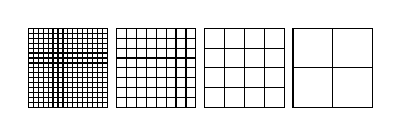
\begin{tikzpicture}
      [>=stealth,
      every node/.style={inner sep=2pt},
      restrict/.style={thick},
      prolong/.style={thick},
      mglevel/.style={rounded rectangle,draw=blue!50!black,fill=blue!20,thick,minimum size=4mm},
      ]
      \begin{scope}\scriptsize
        \newcommand\mgdx{4.0em}
        \newcommand\mgdy{4.0em}
        \newcommand\mgl[1]{(pow(2,#1+1))}
        \newcommand\mgloc[4]{(#1 + #4*\mgdx*#3,#2 + \mgdy*#3)}

        \newcommand\mghx{0.9*\mgdx}
        \newcommand\mghy{0.9*\mgdy}

        \draw[shift=\mgloc{0*\mgdx}{0}{0}{0},
        xstep=\mghy/\mgl{3},
        ystep=\mghy/\mgl{3}]
        (-0.5*\mghy,-0.5*\mghy) grid (0.5*\mghy,0.5*\mghy);

        \draw[shift=\mgloc{1*\mgdx}{0}{0}{0},
        xstep=\mghy/\mgl{2},
        ystep=\mghy/\mgl{2}]
        (-0.5*\mghy,-0.5*\mghy) grid (0.5*\mghy,0.5*\mghy);

        \draw[shift=\mgloc{2*\mgdx}{0}{0}{0},
        xstep=\mghy/\mgl{1},
        ystep=\mghy/\mgl{1}]
        (-0.5*\mghy,-0.5*\mghy) grid (0.5*\mghy,0.5*\mghy);


        \draw[shift=\mgloc{3*\mgdx}{0}{0}{0},
        xstep=\mghy/\mgl{0},
        ystep=\mghy/\mgl{0}]
        (-0.5*\mghy,-0.5*\mghy) grid (0.5*\mghy,0.5*\mghy);
      \end{scope}
    \end{tikzpicture}
    \label{fig:levels}
  \end{figure}
  \textbf{Multigrid} is an $O(n)$ method for solving algebraic problems by defining a hierarchy of scale.
  A multigrid method is constructed from:
  \begin{enumerate}
  \item a series of discretizations
    \begin{itemize}
    \item coarser approximations of the original problem
    \item constructed algebraically or geometrically
    \end{itemize}
  \item intergrid transfer operators
    \begin{itemize}
    \item residual restriction $I_h^H$ (fine to coarse)
    \item state restriction $\hat I_h^H$ (fine to coarse)
    \item partial state interpolation $I_H^h$ (coarse to fine, `prolongation')
    \item state reconstruction $\mathbb{I}_H^h$ (coarse to fine)
    \end{itemize}
  \item Smoothers ($S$)
    \begin{itemize}
    \item correct the high frequency error components
    \item Richardson, Jacobi, Gauss-Seidel, etc.
    \item Gauss-Seidel-Newton or optimization methods
    \end{itemize}
  \end{enumerate}
\end{frame}

\begin{frame}[fragile]
  \frametitle{Multigrid}
  \begin{itemize}
    \item \textbf{Multigrid} methods uses coarse correction for large-scale error
  \end{itemize}
  \begin{figure}
  \centering
  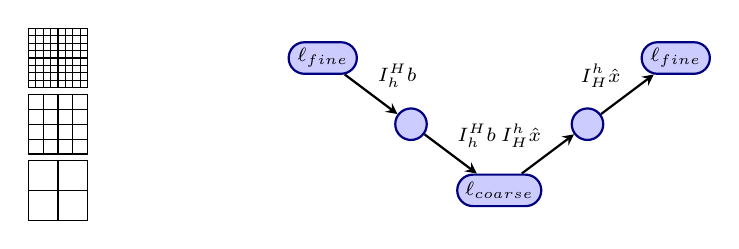
\begin{tikzpicture}
    [>=stealth,
    every node/.style={inner sep=2pt},
    restrict/.style={thick},
    prolong/.style={thick},
    mglevel/.style={rounded rectangle,draw=blue!50!black,fill=blue!20,thick,minimum size=4mm},
    ]
    \begin{scope}\scriptsize
      \newcommand\mgdx{4.0em}
      \newcommand\mgdy{3.0em}
      \newcommand\mgl[1]{(pow(2,#1+1))}
      \newcommand\mgloc[4]{(#1 + #4*\mgdx*#3,#2 + \mgdy*#3)}
      \node[mglevel] (down0) at \mgloc{0}{0}{2}{-1} {\mglevel$_{fine}$};
      \node[mglevel] (down1) at \mgloc{0}{0}{1}{-1} {};
      \node[mglevel] (coarse) at \mgloc{0}{0}{0}{-1} {\mglevel$_{coarse}$};

      \node[mglevel] (up1) at \mgloc{0}{0}{1}{1} {};
      \node[mglevel] (up0) at \mgloc{0}{0}{2}{1} {\mglevel$_{fine}$};

      \path[->,restrict] (down0) edge node [above right] {$\vR\vb$} (down1)
                         (down1) edge node [above right] {$\vR\vb$} (coarse);

      \path[->,prolong] (coarse) edge node [above left] {$\vP\vc$} (up1)
                         (up1) edge node [above left] {$\vP\vc$} (up0);

      %grids
      \newcommand\mghx{0.9*\mgdx}
      \newcommand\mghy{0.9*\mgdy}

      \draw[shift=\mgloc{-5*\mgdx}{0}{2}{0},
      xstep=\mghy/\mgl{2},
      ystep=\mghy/\mgl{2}]
      (-0.5*\mghy,-0.5*\mghy) grid (0.5*\mghy,0.5*\mghy);

      \draw[shift=\mgloc{-5*\mgdx}{0}{1}{0},
      xstep=\mghy/\mgl{1},
      ystep=\mghy/\mgl{1}]
      (-0.5*\mghy,-0.5*\mghy) grid (0.5*\mghy,0.5*\mghy);

      \draw[shift=\mgloc{-5*\mgdx}{0}{0}{0},
      xstep=\mghy/\mgl{0},
      ystep=\mghy/\mgl{0}]
      (-0.5*\mghy,-0.5*\mghy) grid (0.5*\mghy,0.5*\mghy);

  \end{scope}
\end{tikzpicture}
\label{fig:MG}
\end{figure}
Algorithm $MG(\vA,\vb)$ for the solution of $\vA\vx = \vb$:
\begin{align*}
  &\vx = \vS^m(\vx,\vb)             & \text{pre-smooth}\\
  &\vb^{H} = \vR(\vr - \vA\vx)       & \text{restrict residual}\\
  &\vc^{H} = MG(\vR\vA\vP,\vb^{H})   & \text{recurse}\\
  &\vx = \vx + \vP\vc^{H}            & \text{prolong correction}\\
  &\vx = \vx + \vS^n(\vx,\vb)       & \text{post-smooth}\\
\end{align*}

\end{frame}

\begin{comment}
  1. Different schedules of level visit
  2. Full Multigrid -- comes from adaptive mesh refinement
  3. Highly efficient way of arriving at the fine solution
  3. If you have an initial fine level and project right to coarse it's an F-cycle
\end{comment}

\begin{frame}[fragile]
  \frametitle{Full Multigrid(FMG)}
  \begin{figure}
  \centering
  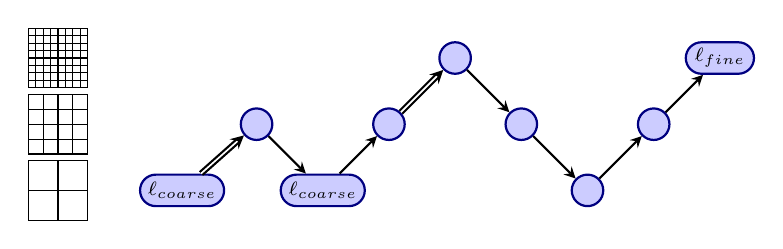
\begin{tikzpicture}
    [>=stealth,
    every node/.style={inner sep=2pt},
    restrict/.style={thick},
    prolong/.style={thick},
    mglevel/.style={rounded rectangle,draw=blue!50!black,fill=blue!20,thick,minimum size=4mm},
    ]
    \begin{scope}\scriptsize
      \newcommand\mgdx{3.0em}
      \newcommand\mgdy{3.0em}
      \newcommand\mgl[1]{(pow(2,#1+1))}
      \newcommand\mgloc[4]{(#1 + #4*\mgdx*#3,#2 + \mgdy*#3)}

      \node[mglevel] (coarseinit) at \mgloc{-3}{0}{0}{0} {$\mglevel_{coarse}$};

      \node[mglevel] (afine) at \mgloc{0}{0}{1}{1} {};

      \node[mglevel] (bcoarse) at \mgloc{2*\mgdx}{0}{0}{1} {$\mglevel_{coarse}$};
      \node[mglevel] (bup1) at \mgloc{2*\mgdx}{0}{1}{1} {};
      \node[mglevel] (bfine) at \mgloc{2*\mgdx}{0}{2}{1} {};

      \node[mglevel] (cdown1) at \mgloc{6*\mgdx}{0}{1}{-1} {};
      \node[mglevel] (ccoarse) at \mgloc{6*\mgdx}{0}{0}{-1} {};
      \node[mglevel] (cup1) at \mgloc{6*\mgdx}{0}{1}{1} {};
      \node[mglevel] (cfine) at \mgloc{6*\mgdx}{0}{2}{1} {$\mglevel_{fine}$};


      \draw[->,restrict,double]
                         (coarseinit) -- node [above right] {} (afine);
      \draw[->,restrict]
                         (afine) -- node [above right] {} (bcoarse);
      \draw[->,restrict]
                         (bcoarse) -- node [above right] {} (bup1);
      \draw[->,restrict,double]
                         (bup1) -- node [above right] {} (bfine);
      \draw[->,restrict]
                         (bfine) -- node [above right] {} (cdown1);
      \draw[->,restrict]
                         (cdown1) -- node [above right] {} (ccoarse);
      \draw[->,restrict]
                         (ccoarse) -- node [above right] {} (cup1);
      \draw[->,restrict]
                         (cup1) -- node [above right] {} (cfine);

      %grids
      \newcommand\mghx{0.9*\mgdx}
      \newcommand\mghy{0.9*\mgdy}

      \draw[shift=\mgloc{-2*\mgdx}{0}{2}{0},
      xstep=\mghy/\mgl{2},
      ystep=\mghy/\mgl{2}]
      (-0.5*\mghy,-0.5*\mghy) grid (0.5*\mghy,0.5*\mghy);

      \draw[shift=\mgloc{-2*\mgdx}{0}{1}{0},
      xstep=\mghy/\mgl{1},
      ystep=\mghy/\mgl{1}]
      (-0.5*\mghy,-0.5*\mghy) grid (0.5*\mghy,0.5*\mghy);

      \draw[shift=\mgloc{-2*\mgdx}{0}{0}{0},
      xstep=\mghy/\mgl{0},
      ystep=\mghy/\mgl{0}]
      (-0.5*\mghy,-0.5*\mghy) grid (0.5*\mghy,0.5*\mghy);

  \end{scope}
\end{tikzpicture}
\label{fig:FMG}
\end{figure}
\begin{itemize}
  \item start wich coarse grid
  \item $\vx$ is prolonged using $\mathbb{I}_H^h$ on first visit to each finer level
  \item truncation error within one cycle
  \item about five work units for many problems
  \item highly efficient solution method
\end{itemize}
\end{frame}

\begin{frame}{$\tau$ formulation of Full Approximation Scheme (FAS)}
  \begin{itemize}
  \item classical formulation: ``coarse grid \emph{accelerates} fine grid $\searrow \nearrow$
  \item $\tau$ formulation: ``fine grid feeds back into coarse grid'' $\nearrow \searrow$
  \item To solve $N u = f$, recursively apply
    \begin{equation*}
      \begin{split}
        \text{pre-smooth} \:\: & \quad \tilde u^h \gets S^h_{\text{pre}}(u^h_0, f^h) \\
        \text{solve coarse problem for $u^H$} \:\: & \quad N^H u^H = \underbrace{I_h^H f^h}_{f^H} + \underbrace{N^H \hat I_h^H \tilde u^h - I_h^H N^h \tilde u^h}_{\tau_h^H} \\
        \text{correction and post-smooth} \:\: & \quad u^h \gets S^h_{\text{post}} \Big( \tilde u^h + I_H^h (u^H - \hat I_h^H \tilde u^h), f^h \Big) \\
      \end{split}
    \end{equation*}
    \begin{tabular}{llll}
      \toprule
      $I_h^H$ & residual restriction & $\hat I_h^H$ & solution restriction \\
      $I_H^h$ & solution interpolation & $f^H = I_h^H f^h$ & restricted forcing \\
      $\{S^h_{\text{pre}},S^h_{\text{post}}\}$ & \multicolumn{3}{l}{smoothing operations on the fine grid} \\
      \bottomrule
    \end{tabular}
  \item At convergence, $u^{H*} = \hat I_h^H u^{h*}$ solves the $\tau$-corrected coarse grid equation
    $N^H u^H = f^H + \tau_h^H$,
    thus $\tau_h^H$ is the ``fine grid feedback'' that makes the coarse grid equation accurate.
  \item $\tau_h^H$ is \emph{local} and need only be recomputed where it becomes stale.
  \end{itemize}
\end{frame}


\begin{frame}{Compatible Relaxation (CR) for $\tau$-FAS}
  \begin{columns}
    \begin{column}{0.5\textwidth}
      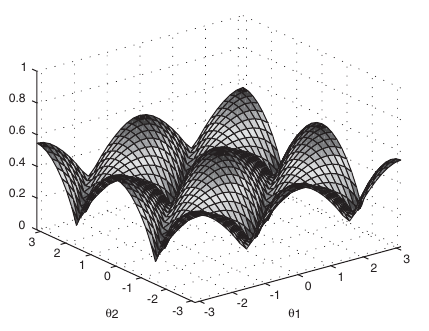
\includegraphics[width=\textwidth]{figures/LivneHabituatedCR} \\
      {\small [Livne 2004]}
    \end{column}
    \begin{column}{0.5\textwidth}
      \begin{itemize}
      \item Reconstructs smooth fine-scale using only coarse solution and forcing term
      \item Apply smoother subject to constraint $\hat I_h^H x = x^H$
        \begin{enumerate}
        \item $x_0 = I_H^h x^H$
        \item $\tilde x_n = x_{n-1} + S_A^{-1}\big(r(x_{n-1}) \big)$
        \item $x_n = \tilde x_n + S_R^{-1}\big(\hat I_h^H \tilde x_n - x^H) \big)$
        \end{enumerate}
      \item Compare to:
        \begin{enumerate}
        \item $x_0 = x_{\text{old}} + I_H^h (x^H - \hat I_h^H x_{\text{old}})$
        %\item  $x_n = x_{n-1} + S_A^{-1}\big( r(\tilde x_{n-1}) \big)$
        \end{enumerate}
      \item Local Fourier Analysis shows slightly slower smoothing for CR
      \end{itemize}
    \end{column}
  \end{columns}
\end{frame}


\begin{frame}{Basic resilience strategy}
  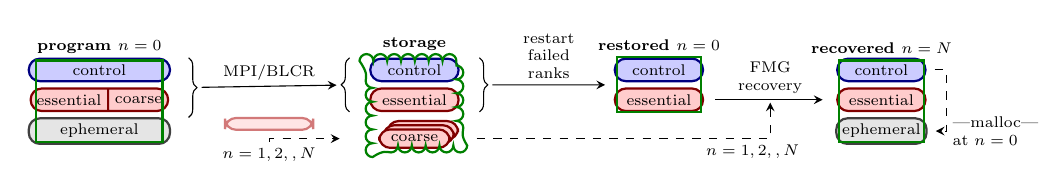
\begin{tikzpicture}
    [scale=0.8,every node/.style={scale=0.8},
    >=stealth,
    control/.style={rectangle,rounded corners,draw=blue!50!black,fill=blue!20,thick,minimum width=5em},
    essential/.style={rectangle,rounded corners,draw=red!50!black,fill=red!20,thick,minimum width=5em},
    ephemeral/.style={rectangle,rounded corners,draw=gray!50!black,fill=gray!20,thick,minimum width=5em},
    statebox/.style={rectangle,draw=green!50!black,thick},
    statetitle/.style={rectangle,draw=green!50!black,fill=green!20,thick},
    storebox/.style={rectangle,draw=},
    rightbrace/.style={decorate,decoration={brace,amplitude=1ex,raise=4pt}},
    leftbrace/.style={decorate,decoration={brace,amplitude=1ex,raise=4pt,mirror}}
    ]
    \scriptsize
    \node[control,minimum width=8em] (progcontrol) {control};
    \node[essential,below=2pt of progcontrol.south,rectangle split,rectangle split parts=2,rectangle split horizontal,minimum width=12em] (progessential) {essential \nodepart{two} coarse};
    \node[ephemeral,minimum width=8em,below=2pt of progessential.south] (progephemeral) {ephemeral};
    \node[statebox,fit=(progcontrol)(progessential)(progephemeral)] (progbox) {};
    \node[above=0pt of progbox.north,anchor=south] {\textbf{program $n=0$}};

    \node[control,right=9em of progcontrol] (storecontrol) {control};
    \node[essential,below=2pt of storecontrol.south] (storeessential) {essential};
    \node[essential,minimum width=4em,below=6pt of storeessential.south, double copy shadow] (storecoarse) {coarse};
    \node[statebox,decorate,decoration={bumps,mirror},fit=(storecontrol)(storecoarse)] (storebox) {};
    \node[above=1pt of storebox.north,anchor=south] {\textbf{storage}};

    \node[control,right=7em of storecontrol] (reccontrol) {control};
    \node[essential,below=2pt of reccontrol.south] (recessential) {essential};
    \node[statebox,fit=(reccontrol)(recessential)] (recbox) {};
    \node[above=0pt of recbox.north,anchor=south] {\textbf{restored $n=0$}};

    \node[control,right=6em of reccontrol] (donecontrol) {control};
    \node[essential,below=2pt of donecontrol.south] (doneessential) {essential};
    \node[ephemeral,below=2pt of doneessential.south] (doneephemeral) {ephemeral};
    \node[statebox,fit=(donecontrol)(doneephemeral)] (donebox) {};
    \node[above=0pt of donebox.north,anchor=south] {\textbf{recovered $n=N$}};

    \draw[decorate,decoration={brace,amplitude=1ex,raise=4pt}] ($(progcontrol.north east) + (3pt,0)$) -- ($(progephemeral.north east) + (3pt,0)$) node[midway,xshift=1ex] (progbrace) {};
    \draw[leftbrace] ($(storecontrol.north west) - (4pt,0)$) -- ($(storeessential.south west) - (4pt,0)$) node[midway,xshift=-1ex] (storebrace) {};
    \draw[rightbrace] ($(storecontrol.north east) + (4pt,0)$) -- ($(storeessential.south east) + (4pt,0)$) node[midway,xshift=1ex] (storerbrace) {};
    \draw[->,shorten >=4pt,shorten <=4pt] (progbrace) -- (storebrace) node[midway,above] (midarrow) {MPI/BLCR};

    \node[below=1.4em of midarrow,essential,draw=red!50!gray!70,fill=red!10] (coarserun) {};
    \draw[->,dashed,shorten >=14pt,shorten <=4pt] (coarserun) |- (storecoarse) node [near start,below,yshift=-3pt] {\scriptsize $n=1,2,\dotsc,N$};
    \draw[->,shorten >=4pt,shorten <=4pt] (storerbrace) -- (recbox.west) node[midway,above,text width=5em,align=center] (midarrow) {restart failed ranks};
    \draw[->,shorten >=5pt,shorten <=4pt] (recessential.east) -- (doneessential) node[midway,above,text width=5em,align=center] (fmgrecover) {FMG recovery};
    \draw[->,dashed,shorten >=1pt,shorten <=3pt] ($(storecoarse.east) + (1em,0)$) -| (fmgrecover) node[midway,below,xshift=-1em] {\scriptsize $n=1,2,\dotsc,N$};
    \draw[->,dashed,shorten >=3pt,shorten <=3pt] (donecontrol.east) -| ($(donecontrol.east) + (3ex,0)$) |- (doneephemeral.east) node[midway,right,text width=4em] {\cverb|malloc| at $n=0$};
  \end{tikzpicture}
\begin{description}
\item[control] contains program stack, solver configuration, etc.
\item[essential] program state that cannot be easily reconstructed: time-dependent solution, current optimization/bifurcation iterate
\item[ephemeral] easily recovered structures: assembled matrices, preconditioners, residuals, Runge-Kutta stage solutions
\end{description}
\begin{itemize}
\item Essential state at time/optimization step $n$ is \alert{inherently globally coupled} to step $n-1$ (otherwise we could use an explicit method)
\item \emph{Coarse} level checkpoints are orders of magnitude smaller, but allow rapid recovery of essential state
\item FMG recovery needs only \alert{nearest neighbors}
\end{itemize}
\end{frame}

\begin{frame}[fragile]{Multiscale compression and recovery using $\tau$ form}
   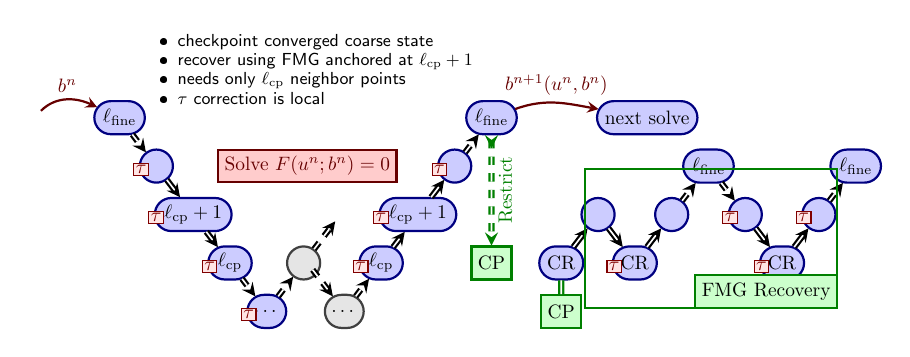
\begin{tikzpicture}
    [scale=0.7,every node/.style={scale=0.7},
    >=stealth,
    restrict/.style={thick,double},
    prolong/.style={thick,double},
    cprestrict/.style={green!50!black,thick,double,dashed},
    control/.style={rectangle,red!40!black,draw=red!40!black,thick},
    mglevel/.style={rounded rectangle,draw=blue!50!black,fill=blue!20,thick,minimum size=6mm},
    checkpoint/.style={rectangle,draw=green!50!black,fill=green!20,thick,minimum size=6mm},
    mglevelhide/.style={rounded rectangle,draw=gray!50!black,fill=gray!20,thick,minimum size=6mm},
    tau/.style={text=red!50!black,draw=red!50!black,fill=red!10,inner sep=1pt},
    crelax/.style={text=green!50!black,fill=green!10,inner sep=0pt}
    ]
    \begin{scope}
      \newcommand\mgdx{1.9em}
      \newcommand\mgdy{2.5em}
      \newcommand\mgloc[4]{(#1 + #4*\mgdx*#3,#2 + \mgdy*#3)}
      \node[mglevel] (fine0) at \mgloc{0}{0}{4}{-1} {\mglevelfine};
      \node[mglevel] (finem1down0) at \mgloc{0}{0}{3}{-1} {};
      \node[mglevel] (cp1down0) at \mgloc{0}{0}{2}{-1} {$\mglevelcp+1$};
      \node[mglevel] (cpdown0) at \mgloc{0}{0}{1}{-1} {\mglevelcp};
      \node[mglevel] (coarser0) at \mgloc{0}{0}{0}{0} {\ldots};

      \node[mglevelhide] (cpup0) at \mgloc{0}{0}{1}{1} {};
      \node (cp1up0) at \mgloc{0}{0}{2}{1} {};

      \node (cpdown1) at \mgloc{4em}{0}{1}{-1} {};
      \node[mglevelhide] (coarser1) at \mgloc{4em}{0}{0}{1} {\ldots};
      \node[mglevel] (cpup1) at \mgloc{4em}{0}{1}{1} {\mglevelcp};
      \node[mglevel] (cp1up1) at \mgloc{4em}{0}{2}{1} {$\mglevelcp+1$};
      \node[mglevel] (finem1up1) at \mgloc{4em}{0}{3}{1} {};
      \node[mglevel] (fine1) at \mgloc{4em}{0}{4}{1} {\mglevelfine};

      \draw[->,restrict,dashed] (fine0) -- (finem1down0);
      \draw[->,restrict] (finem1down0) -- (cp1down0);
      \draw[->,restrict] (cp1down0) -- (cpdown0);
      \draw[->,restrict,dashed] (cpdown0) -- (coarser0);
      \draw[->,prolong,dashed] (coarser0) -- (cpup0);
      \draw[->,prolong,dashed] (cpup0) -- (cp1up0);

      \draw[->,restrict,dashed] (cpdown1) -- (coarser1);
      \draw[->,prolong,dashed] (coarser1) -- (cpup1);
      \draw[->,prolong] (cpup1) -- (cp1up1);
      \draw[->,prolong] (cp1up1) -- (finem1up1);
      \draw[->,prolong,dashed] (finem1up1) -- (fine1);

      \node[checkpoint] at (4em + \mgdx*4,\mgdy) (cp) {CP};
      \draw[>->,cprestrict] (fine1) -- node[below,sloped] {Restrict} (cp);

      \node[left=\mgdx of fine0] (bnanchor) {};
      \node[control,fill=red!20] at (1.1*\mgdx,3*\mgdy) {Solve $F(u^n;b^n) = 0$};
      \node[mglevel,right=of fine1] (finedt) {next solve};
      \draw[->, >=stealth, control] (fine1) to[out=20,in=170] node[above] {$b^{n+1}(u^n,b^n)$} (finedt);
      \draw[->, >=stealth, control] (bnanchor) to[out=45,in=155] node[above] {$b^n$} (fine0);

      % Recovery process
      \begin{scope}[xshift=8*\mgdx]
        \node[checkpoint] (rcp) at \mgloc{0}{0}{0}{0} {CP};
        \node[mglevel] (r0a) at \mgloc{0}{\mgdy}{0}{0} {CR};
        \node[mglevel] (r1a) at \mgloc{0}{\mgdy}{1}{1} {};
        \node[mglevel] (r0b) at \mgloc{2*\mgdx}{\mgdy}{0}{0} {CR};
        \node[mglevel] (r1b) at \mgloc{2*\mgdx}{\mgdy}{1}{1} {};
        \node[mglevel] (r2b) at \mgloc{2*\mgdx}{\mgdy}{2}{1} {\mglevelfine};
        \node[mglevel] (r1c) at \mgloc{6*\mgdx}{\mgdy}{1}{-1} {};
        \node[mglevel] (r0d) at \mgloc{6*\mgdx}{\mgdy}{0}{0} {CR};
        \node[mglevel] (r1d) at \mgloc{6*\mgdx}{\mgdy}{1}{1} {};
        \node[mglevel] (r2d) at \mgloc{6*\mgdx}{\mgdy}{2}{1} {\mglevelfine};

        \draw[-,prolong,green!50!black] (rcp) -- (r0a);
        \draw[->,prolong] (r0a) -- (r1a);
        \draw[->,restrict] (r1a) -- (r0b);
        \draw[->,restrict] (r0b) -- (r1b);
        \draw[->,restrict,dashed] (r1b) -- (r2b);
        \draw[->,restrict,dashed] (r2b) -- (r1c);
        \draw[->,restrict] (r1c) -- (r0d);
        \draw[->,restrict] (r0d) -- (r1d);
        \draw[->,restrict,dashed] (r1d) -- (r2d);

        \foreach \smooth in {finem1down0, cp1down0, cpdown0, coarser0,
          cpup1, cp1up1, finem1up1,
          r0b,r1c,r0d,r1d} {
          \node[above left=-5pt of \smooth.west,tau] {$\tau$};
        }
        \node[rectangle,fill=none,draw=green!50!black,thick,fit=(rcp)(r2d)] (recoverbox) {};
        \node[rectangle,draw=green!50!black,fill=green!20,thick,minimum size=6mm,above={0cm of recoverbox.south east},anchor=south east] (recover) {FMG Recovery};
      \end{scope}
      \node (notation) at (\mgdx,5*\mgdy) {
        \begin{minipage}{18em}\small\sf
          \begin{itemize}\addtolength{\itemsep}{-5pt}
          \item checkpoint converged coarse state
          \item recover using FMG anchored at $\mglevelcp+1$
          \item needs only $\mglevelcp$ neighbor points
          \item $\tau$ correction is local
          \end{itemize}
        \end{minipage}
      };
    \end{scope}
  \end{tikzpicture}
  \begin{itemize}
  \item Normal multigrid cycles visit all levels moving from $n \to n+1$
  \item FMG recovery only accesses levels finer than $\ell_{CP}$
  \item Only failed processes and neighbors participate in recovery
  \item Lightweight checkpointing for transient adjoint computation
  \item Postprocessing applications, e.g., in-situ visualization at high temporal resolution in part of the domain
  \end{itemize}
\end{frame}

\begin{frame}{First-order cost model for FAS resilience}
  Extend first-order locality-unaware model of Young (1974):
  \begin{description}
  \item[$\timeW$] time to write a heavy fine-grid checkpointed state
  \item[$\timeR$] time to read back lost state
  \item[$R$] fraction of forward simulation needed for recomputation from a saved state
  \item[$P$] the heavy checkpoint interval
  \item[$M$] mean time to failure
  \end{description}
  Neglect cost of I/O for lightweight coarse-grid checkpoints
  \begin{equation}\label{eq:overhead}
    \text{Overhead} = 1 - \text{AppUtilization} = \underbrace{\frac{\timeW}{P}}_{\text{writing}}
    + \underbrace{\frac{\timeR}{M}}_{\text{reading after failure}}
    + \underbrace{\frac{R P}{2M}}_{\text{recomputation}}
  \end{equation}
  Minimized for a heavy checkpointing interval $P = \sqrt{2 M \timeW / R}$
  \begin{equation}\label{eq:minoverhead}
    \text{Overhead}^* = \sqrt{2 \timeW R / M} + \timeR / M
    % $ \text{Overhead}^* = \sqrt{\frac{2 \timeW R}{M}} + \frac{\timeR}{M} $,
  \end{equation}
  where the first term is always larger than the second.
  Conventional checkpointing schemes store only fine-grid state, thus $R=1$ (recovery costs the same as initial computation).
\end{frame}

\begin{frame}[fragile]
  \frametitle{Redundant Coarse-Grid Error Detection}
  A redundant coarse problem may be used to trivially check for errors:
  \begin{figure}
    \centering
    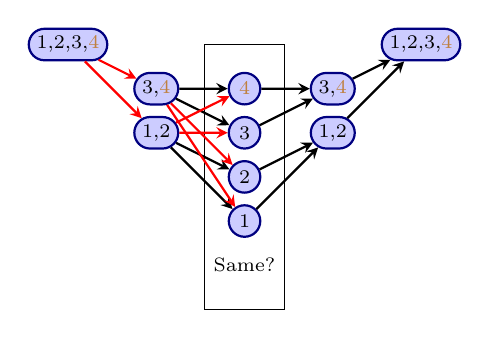
\begin{tikzpicture}
      [>=stealth,
      every node/.style={inner sep=2pt},
      restrict/.style={thick},
      prolong/.style={thick},
      mglevel/.style={rounded rectangle,draw=blue!50!black,fill=blue!20,thick,minimum size=4mm},
      ]
      \begin{scope}\scriptsize
        \newcommand\mgdx{4.0em}
        \newcommand\mgdy{4.0em}
        \newcommand\mgl[1]{(pow(2,#1+1))}
        \newcommand\mgloc[4]{(#1 + #4*\mgdx*#3,#2 + \mgdy*#3)}
        \node[mglevel] (down0) at \mgloc{0}{0}{2}{-1} {\red{1},\green{2},\blue{3},\color{brown}{4}};

        \node[mglevel] (down10) at \mgloc{0}{0}{1}{-1} {\red{1},\green{2}};
        \node[mglevel] (down11) at \mgloc{0}{0.5*\mgdy}{1}{-1} {\blue{3},\color{brown}{4}};

        \node[mglevel] (coarse0) at \mgloc{0}{0}{0}{-1} {\red{1}};
        \node[mglevel] (coarse1) at \mgloc{0}{0.5*\mgdy}{0}{-1} {\green{2}};
        \node[mglevel] (coarse2) at \mgloc{0}{1.0*\mgdy}{0}{-1} {\blue{3}};
        \node[mglevel] (coarse3) at \mgloc{0}{1.5*\mgdy}{0}{-1} {\color{brown}{4}};

        \node[] (same) at \mgloc{0}{-0.5*\mgdy}{0}{-1} {Same?};

        \draw \mgloc{-0.45*\mgdx}{-1.0*\mgdy}{0}{0} rectangle \mgloc{0.45*\mgdx}{2.0*\mgdy}{0}{0};

        \node[mglevel] (up10) at \mgloc{0}{0}{1}{1} {\red{1},\green{2}};
        \node[mglevel] (up11) at \mgloc{0}{0.5*\mgdy}{1}{1} {\blue{3},\color{brown}{4}};

        \node[mglevel] (up0) at \mgloc{0}{0}{2}{1} {\red{1},\green{2},\blue{3},\color{brown}{4}};

        \draw[->,restrict,red] (down0) -- (down10);
        \draw[->,restrict,red] (down0) -- (down11);

        \draw[->,restrict] (down10) -- (coarse0);
        \draw[->,restrict] (down10) -- (coarse1);

        \draw[->,restrict] (down11) -- (coarse2);
        \draw[->,restrict] (down11) -- (coarse3);

        % comm
        \draw[->,restrict,red] (down11) -- (coarse0);
        \draw[->,restrict,red] (down11) -- (coarse1);
        \draw[->,restrict,red] (down10) -- (coarse2);
        \draw[->,restrict,red] (down10) -- (coarse3);

        \draw[->,restrict] (coarse0) -- (up10);
        \draw[->,restrict] (coarse1) -- (up10);
        \draw[->,restrict] (coarse2) -- (up11);
        \draw[->,restrict] (coarse3) -- (up11);

        \draw[->,restrict] (up10) -- (up0);
        \draw[->,restrict] (up11) -- (up0);

      \end{scope}
    \end{tikzpicture}
    \label{fig:RedundantMGTest}
  \end{figure}
  However, this is uninteresting and doesn't exploit the algorithm; can we do anything better?
\end{frame}

\begin{frame}[fragile]
  \frametitle{$\tau$-Correction Error Detection}
  \begin{block}{Recall}
      At convergence, $u^{H*} = \hat I_h^H u^{h*}$ solves the $\tau$-corrected coarse grid equation
    $N^H u^H = f^H + \tau_h^H$,
    thus $\tau_h^H$ is the ``fine grid feedback'' that makes the coarse grid equation accurate.
  \end{block}
  \begin{figure}
    \centering
  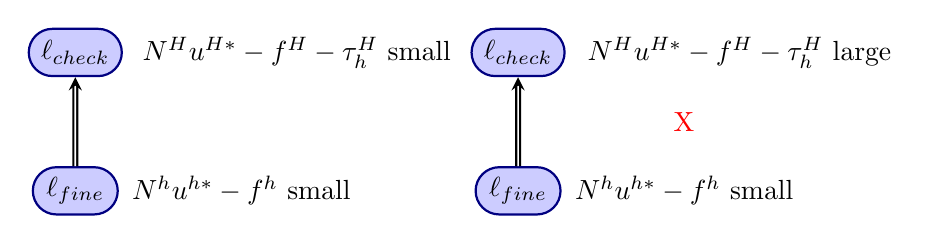
\begin{tikzpicture}
    [>=stealth,
    restrict/.style={thick,double},
    prolong/.style={thick,double},
    cprestrict/.style={green!50!black,thick,double,dashed},
    control/.style={rectangle,red!40!black,draw=red!40!black,thick},
    mglevel/.style={rounded rectangle,draw=blue!50!black,fill=blue!20,thick,minimum size=6mm},
    checkpoint/.style={rectangle,draw=green!50!black,fill=green!20,thick,minimum size=6mm},
    mglevelhide/.style={rounded rectangle,draw=gray!50!black,fill=gray!20,thick,minimum size=6mm},
    tau/.style={text=red!50!black,draw=red!50!black,fill=red!10,inner sep=1pt},
    crelax/.style={text=green!50!black,fill=green!10,inner sep=0pt}
    ]
    \newcommand\mgdx{2.0em}
    \newcommand\mgdy{2.5em}
    \newcommand\mgloc[4]{(#1 + #4*\mgdx*#3,#2 + \mgdy*#3)}
    \begin{scope}
      \node[mglevel] (fineright) at \mgloc{0}{0}{0}{0} {\mglevel$_{fine}$};
      \node[mglevel] (checkright) at \mgloc{0}{0}{2}{0} {\mglevel$_{check}$};
      \draw[->,restrict] (fineright) -- (checkright);

      \node[] (finerightnorm) at \mgloc{3*\mgdx}{0}{0}{0} {$\abs{N^h u^{h*} - f^h}$ small};
      \node[] (coarserightnorm) at \mgloc{4.0*\mgdx}{0}{2}{0} {$\abs{N^H u^{H*} - f^H - \tau_h^H}$ small};

      \node[mglevel] (finewrong) at \mgloc{8*\mgdx}{0}{0}{0} {\mglevel$_{fine}$};
      \node[mglevel] (checkwrong) at \mgloc{8*\mgdx}{0}{2}{0} {\mglevel$_{check}$};
      \draw[->,restrict] (finewrong) -- (checkwrong);

      \node[] (finewrongnorm) at \mgloc{11*\mgdx}{0}{0}{0} {$\abs{N^h u^{h*} - f^h}$ small};
      \node[] (coarsewrongnorm) at \mgloc{12.0*\mgdx}{0}{2}{0} {$\abs{N^H u^{H*} - f^H - \tau_h^H}$ large};

      \node[green] (OK) at \mgloc{3*\mgdx}{0}{1}{0} {\checkmark};
      \node[red] (BAD) at \mgloc{11*\mgdx}{0}{1}{0} {X};

    \end{scope}
  \end{tikzpicture}
  \end{figure}
  \begin{itemize}
  \item \emph{Local} detection if $\abs{N^H u^{H*} - f^H - \tau_h^H}$ is large
  \item incorrect result indicates error in fine grid residual evaluation (likely), restriction, or coarse grid residual.
  \end{itemize}
\end{frame}


\begin{frame}{Reducing memory bandwidth}
  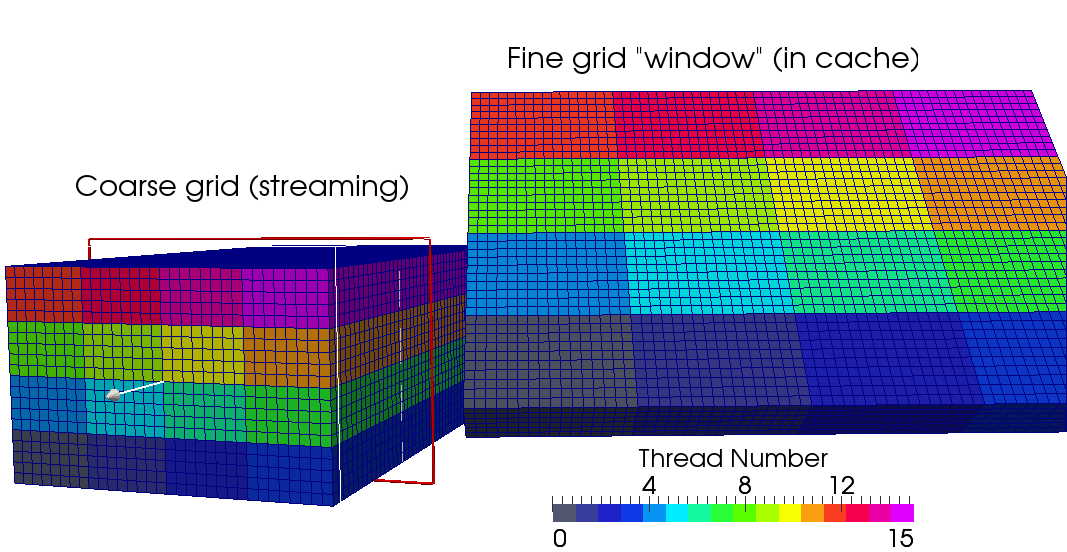
\includegraphics[width=\textwidth]{figures/MG/SRMGWindow}
  \begin{itemize}
  \item Sweep through ``coarse'' grid with moving window
  \item Zoom in on new slab, construct fine grid ``window'' in-cache
  \item Interpolate to new fine grid, apply pipelined smoother ($s$-step)
  \item Compute residual, accumulate restriction of state and residual into coarse grid, expire slab from window
  \end{itemize}
\end{frame}

\begin{frame}{Arithmetic intensity of sweeping visit}
  \begin{itemize}
  \item Assume 3D cell-centered, 7-point stencil
  \item 14 flops/cell for second order interpolation
  \item $\ge 15$ flops/cell for fine-grid residual or point smoother
  \item 2 flops/cell to enforce coarse-grid compatibility
  \item 2 flops/cell for plane restriction
  \item assume coarse grid points are reused in cache
  \item Fused visit reads $u^H$ and writes $\hat I_h^H u^h$ and $I_h^H r^h$
  \item Arithmetic Intensity
    \begin{equation}
      \frac{{\overbrace{15}^{\text{interp}}} + {\overbrace{2\cdot (15+2)}^{\text{compatible relaxation}}} + \overbrace{2\cdot 15}^{\text{smooth}} + \overbrace{15}^{\text{residual}} + \overbrace{2}^{\text{restrict}}}{3 \cdot \texttt{sizeof(scalar)} / \underbrace{2^3}_{\text{coarsening}}} \gtrsim 30
    \end{equation}
  \end{itemize}
\end{frame}

\begin{frame}{Regularity}
  Accuracy of recovery depends on operator regularity
  \begin{itemize}
  \item Even with regularity, we can only converge up to discretization error, unless we add a \emph{consistent} fine-grid residual evaluation
  \item Visit fine grid with some overlap, but patches do not agree exactly in overlap
  \item Need decay length for high-frequency error components (those that restrict to zero) that is bounded with respect to grid size
  \item Required overlap $J$ is proportional to the number of cells to cover decay length
  \item Can enrich coarse space along boundary, but causes loss of coarse-grid sparsity
  \item Brandt and Diskin (1994) has two-grid LFA showing $J \lesssim 2$ is sufficient for Laplacian
  \item With $L$ levels, overlap $J(k)$ on level $k$,
    \begin{equation*}
      2J(k) \ge s (L-k+1)
    \end{equation*}
    where $s$ is the smoothness order of the solution or the discretization order (whichever is smaller)
  \end{itemize}
\end{frame}

\begin{frame}{$\tau$-FAS and multiscale modeling}
  \begin{itemize}
  \item Systematic Upscaling/Renormalization Multigrid (Brandt, Ron)
    \begin{description}
    \item[interpolation] initialize microscale variables to be (at least statistically) compatible with macro variables
    \item[equilibriation] local processing to evolve microscale variables toward a local equilibrium
    \item[restriction] sample microscale solution and residual to correct macro model
    \end{description}
  \item Heterogeneous Multiscale Method (E and Engquist, 2003)
    \begin{description}
    \item[reconstruction] initialize micro model
    \item[constrained micro model] evolve micro model, constrained by compatibility with macro model
    \item[compression] statistical data estimator
    \end{description}
  \item Sequential vs concurrent scale coupling
  \item Further comparison in E, \textit{The Heterogeneous Multiscale Method and the ``Equation-free'' Approach to Multiscale Modeling, 2012}.
  \item Many applications: electronic structure, oscillatory integro-differential equations, high-frequency wave propagation, statistical mechanics, complex fluids, image processing, etc.
  \end{itemize}
\end{frame}

\begin{frame}{Cool Topics in Multiscale Computation}
  \begin{multicols}{2}
    \begin{itemize}
    \item Solve PDE in fewer flops than evaluating an analytic solution
    \item Solve PDE in $\bigO(\abs{\log n}\abs{\log \epsilon}^d)$ memory
    \item Compute $k$ eigenvalues in $\bigO(n \log k)$
    \item Project vector onto eigenbasis in $\bigO(n \log k)$
    \item Optimal-order graph partitioning and clustering
    \item Continuation and transient problems without revisiting fine grid
    \item Global optimization without sacrificing optimality, ``multiscale annealing''
    \item Accelerate Monte-Carlo slowdown due to spuriously correlated sampling
    \end{itemize}
  \end{multicols}
\end{frame}


\end{document}
